\section{Применение локальных оценок константы Гёльдера для ускорения сходимости АГП}
В части работы будем рассматривать задачу глобальной оптимизации в постановке без функциональных ограничений.
Как видно из описания метода, независимо от локальных свойств оптимизируемой одномерной
функции, для вычисления характеристик всех интервалов (\ref{step3_1}) используется одно и то же
значение оценки константы Гёльдера (\ref{step2}). В работе \cite{sergLocalTuningFirst} было предложено использовать различные
значения \(M=\mu_1\) (\(\mu_1\) из (\ref{step2}) в случае отсутствия функциональных ограничений), (\ref{step3_1})) для каждого интревала, а
также показана эффективность такого подхода в случае одномерной оптимизации функций,
удовлетворяющих условию Липшица. В работе \cite{nestedLocal} рассмотрено применение
адаптивных оценок констант Липшица в схеме многомерной вложенной оптимизации.

Для каждого интревала локальная оценка константы является максимум-аддитивной свёрткой
<<глобальной>> и <<локальной>> компонент (\(\gamma\) и \(\lambda\) соответственно):
\begin{displaymath}
  \begin{array}{lr}
    \lambda_i=\max\{H_{i-1},H_i,H_{i+1}\} \\
    H_i=\frac{|z_i-z_{i-1}|}{\Delta_i} \\
    H^k=\max\{H_i:i=2,\dots ,k\} \\
    \gamma_i=H^k\frac{\Delta_i}{\Delta^{max}} \\
    \Delta^{max}=\max\{\Delta_{i}:i=2,\dots ,k\}
  \end{array}
\end{displaymath}
\begin{equation}
\label{additiveConv}
M_i=r\cdot \max\{H_i, \frac{1}{2}(\lambda_i+\gamma_i),\xi\}
\end{equation}

Параметр \(\xi\) предотвращает обнуление оценки \(M_i\) в случае, если оптимизируемая
фнкция является тождественной константой, и выбирается достаточно малым.
Данный вариант свёртки не зависит от параметра \(r\), однако в \cite{sergLocalTuning}
также рассматриваетсяи адаптивная свёртка:
\begin{equation}
\label{additiveAdaptiveConv}
M_i=r\cdot \max\{H_i, \frac{\lambda_i}{r}+\frac{r-1}{r}\gamma_i,\xi\}
\end{equation}

Если априори известно, что оптимизируемая функция имеет сложный рельеф с множеством
локальных минимумов, то \(r\) изначально задаётся большим, что ведёт к преобладанию в
адаптивной свёртке «глобальной» сооставляющей \(\gamma\).

Оба варианта свёртки (\ref{additiveConv}), (\ref{additiveAdaptiveConv}) были предложены
и детально рассмотрены в \cite{sergLocalTuning} для случая одномерных функций,
удовлетворяющих условию Липшица. В данном разделе будет рассмотрено применение этих
свёрток для оптимизации двумерных функций в случае редукции размерности с помощью развёрток.

В \cite{sergLocalTuning} приведена теорема о сходимости метода в случае, если целевая функция
липшицева, однако, как правило, подобные утверждения справедливы и в Гёльдеровой метрике, поэтому,
предположительно, будет верна следующая гепотеза:
\begin{hypothesis}
Пусть целевая функция \(f(x)\) удовлетвворяет условию Гёльдера с конечной константой
\(H > 0\), и пусть \(x\) является предельной точкой последовательности \(\{x_k\}\),
порождаемой алгоритмом. Тогда верны следующие утверждения:
\begin{enumerate}
  \item Если \(x\in(0;1)\), то сходимость к точке \(x\) является двухсторонней, т.е.
  существуют две подпоследовательности \(\{x_k\}\), сходящиеся к \(x\): одна слева,
  а другая справа;
  \item \(f(x_k) \geqslant f(x)\) для всех точек испытаний \(x_k, k \geqslant 1\);
  \item Если существует другая предельна точка \(x^* = x\), то \(f(x) = f(x^*)\);
  \item Если функция \(f(x)\) имеет конечное число локальных минимумов на отрезке \([0, 1]\),
  то точка \(x\) является локально оптимальной;
  \item (Существенное условие сходимости к глобальномк минимуму). Пусть \(x^*\)
  является глобальным минимумом \(f(x)\). Если существует такое число \(k^*\),
  что для всех итераций с номерами \(k > k^*\) неравенство
  \(M_j(k) > H_j(k)\) выполняется, где \(H_j(k)\) --- это константа Гёльдера на интервале
  \([x_{j(k)-1}, x_{j(k)}]\), содержащем \(x^*\), а \(M_{j(k)}\) её оценка.
  Тогда множество предельных точек последовательности \(\{x_k\}\) совпадает с множеством
  глобальных минимумов функции \(f(x)\).
\end{enumerate}
\end{hypothesis}

Доказательство гепотезы требует отдельных теоретических исследований. В рамках данной
работы оно не будет проведено, наличие сходимости установлено только численно.

Эксперименты по оценке эффективности метода с локально-адаптивной оценкой константы
Гёльдера производились на двумерных классах задач Гришагина (\(F_{GR}\))
и GKLS Simple 2d, упомянутых в разделе \ref{subsec:test_problems}
Каждый из классов содержит 100 многоэкстремальных функций. Развёртка во всех экспериментах
строилась с плотностью \(m=12\), параметр \(\varepsilon\) в критерии остановки был равен \(10^{-3}\).
Параметр \(r\) выбирался минимально возможным, при котором заданный метод решает все
задачи класса. Шаг поиска \(r\) равен \(0.1\).

\begin{figure}[ht]
    \centering
    \subfloat[глобальная оценка \(H\)]{{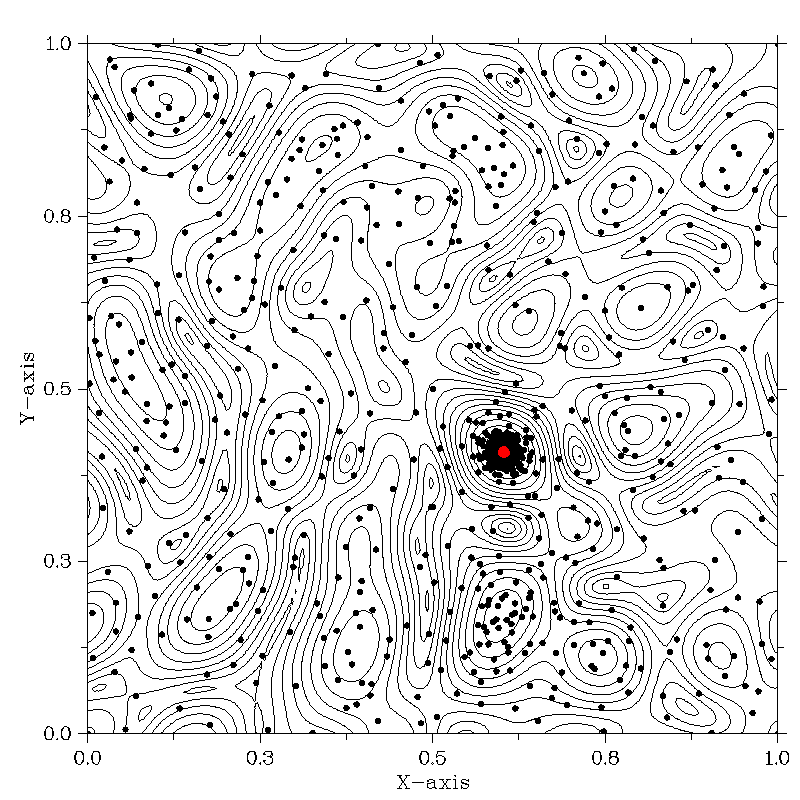
\includegraphics[width=0.45\textwidth]{images/gs_glob.png} }}
    \qquad
    \subfloat[локально-адаптивная оценка \(H\)]{{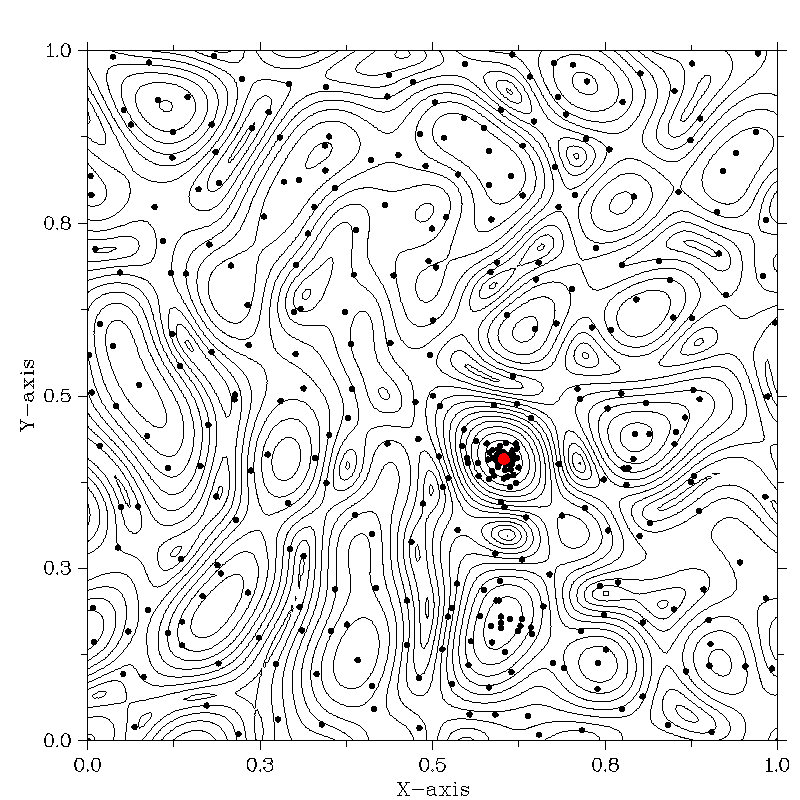
\includegraphics[width=0.45\textwidth]{images/gs_loc.png} }}
    \caption{Линии уровня одной из функций класса \(F_{GR}\)}
    \label{fig:grish_isolines}
\end{figure}

Для наглядной иллюстрации преимущества локально-адаптивной схемы оценки константы
\(H\) рассмотрим результаты работы метода на конкретном примере. На рис. \ref{fig:grish_isolines} показаны
линии уровня одной из функций класса \(F_{GR}\) и точки испытаний, проведённых методом с глобальной
оценкой константы Гёльдера и с оценкой по формуле (\ref{additiveConv}). Как видно из рисунков, метод с
глобальной оценкой константы проводит большое число испытаний в окрестности точки
глобального минимума прежде (всего проведено 1086 испытаний), чем выполнится условие
остановки, в то врямя, как метод с локально-адаптивной оценкой гораздо быстрее
сходится (всего проведено 385 испытаний). Аналогичная ситуация имеет место при
оптимизации одной из функций класса GKLS Simple 2d (рис. \ref{fig:gkls_isolines}). Метод с глобальной
оценкой константы произвёл 2600 испытаний, а метод с локально-адаптивной оценкой – 1190.

\begin{figure}[ht]
    \centering
    \subfloat[глобальная оценка \(H\)]{{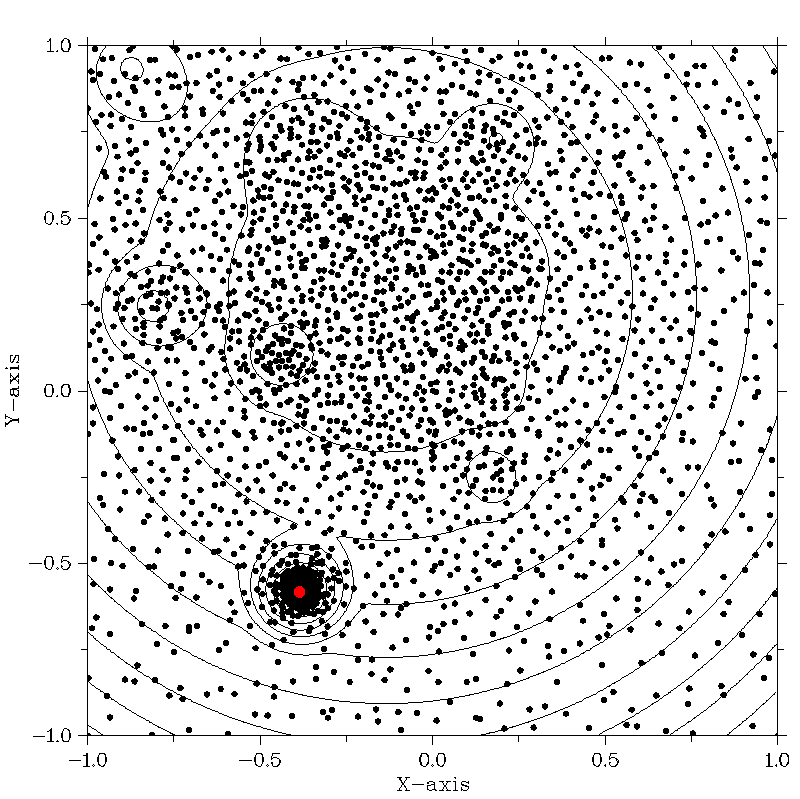
\includegraphics[width=0.45\textwidth]{images/gkls_glob.png} }}
    \qquad
    \subfloat[локально-адаптивная оценка \(H\)]{{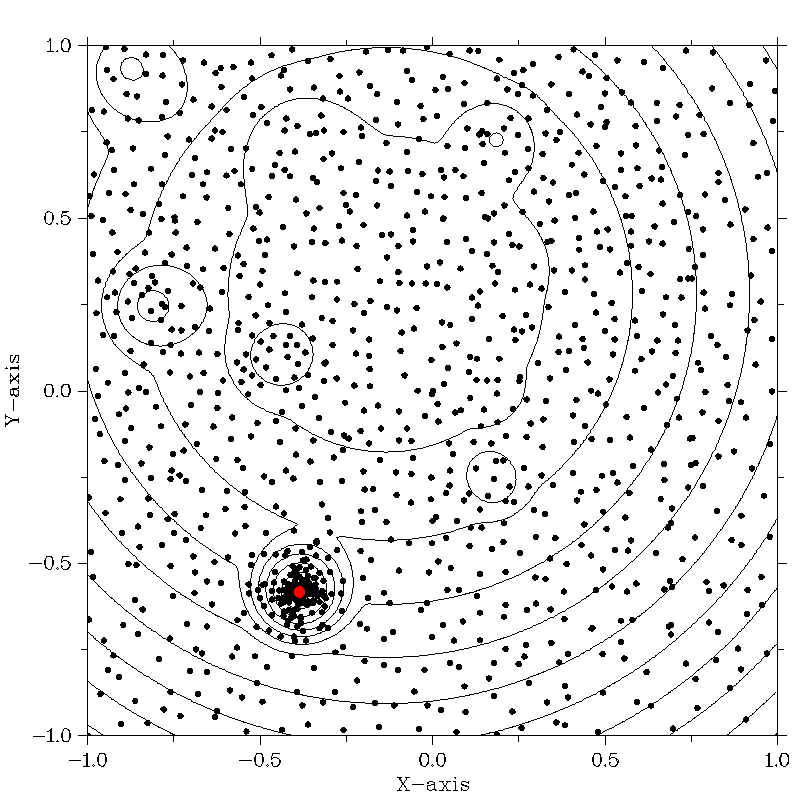
\includegraphics[width=0.45\textwidth]{images/gkls_loc.png} }}
    \caption{Линии уровня одной из функций класса GKLS Simple 2d}
    \label{fig:gkls_isolines}
\end{figure}

\begin{figure}[ht]
    \center
    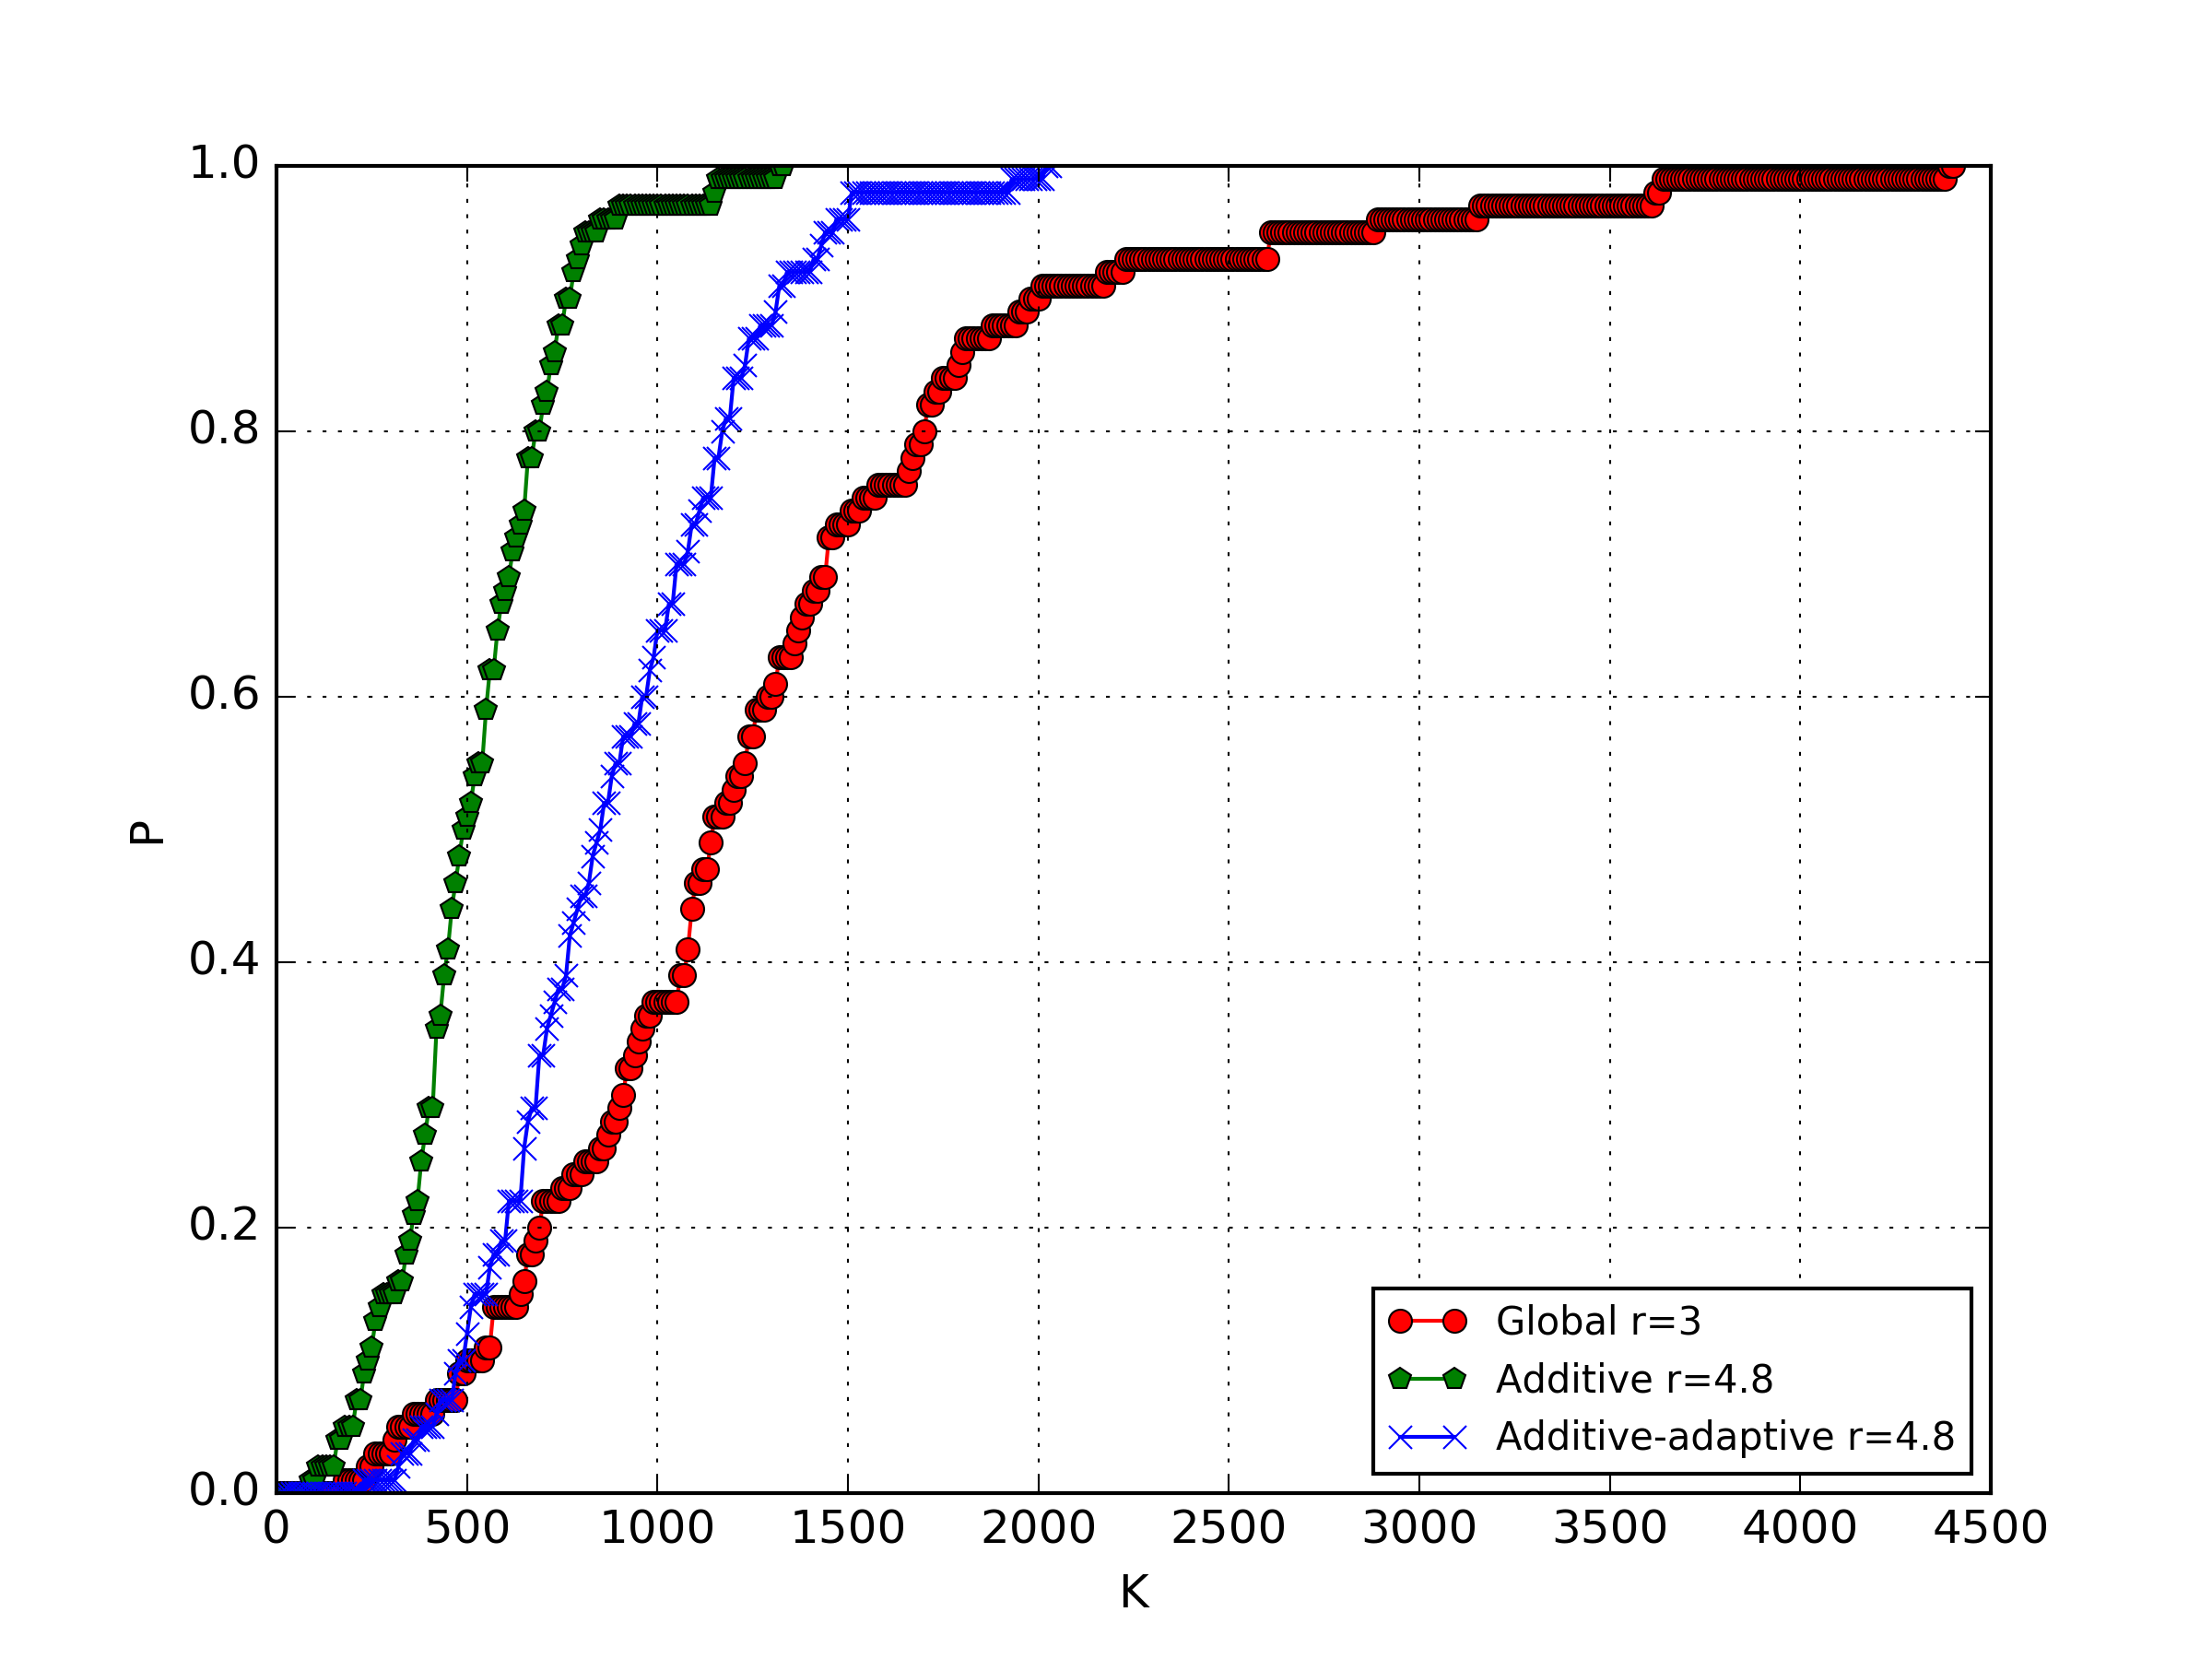
\includegraphics[width=0.75\textwidth]{images/grishagin.png}
    \caption{Операционные характеристики методов на классе задач \(F_{GR}\)}
    \label{fig:grishh_op}
\end{figure}

\begin{figure}[H]
  \center
  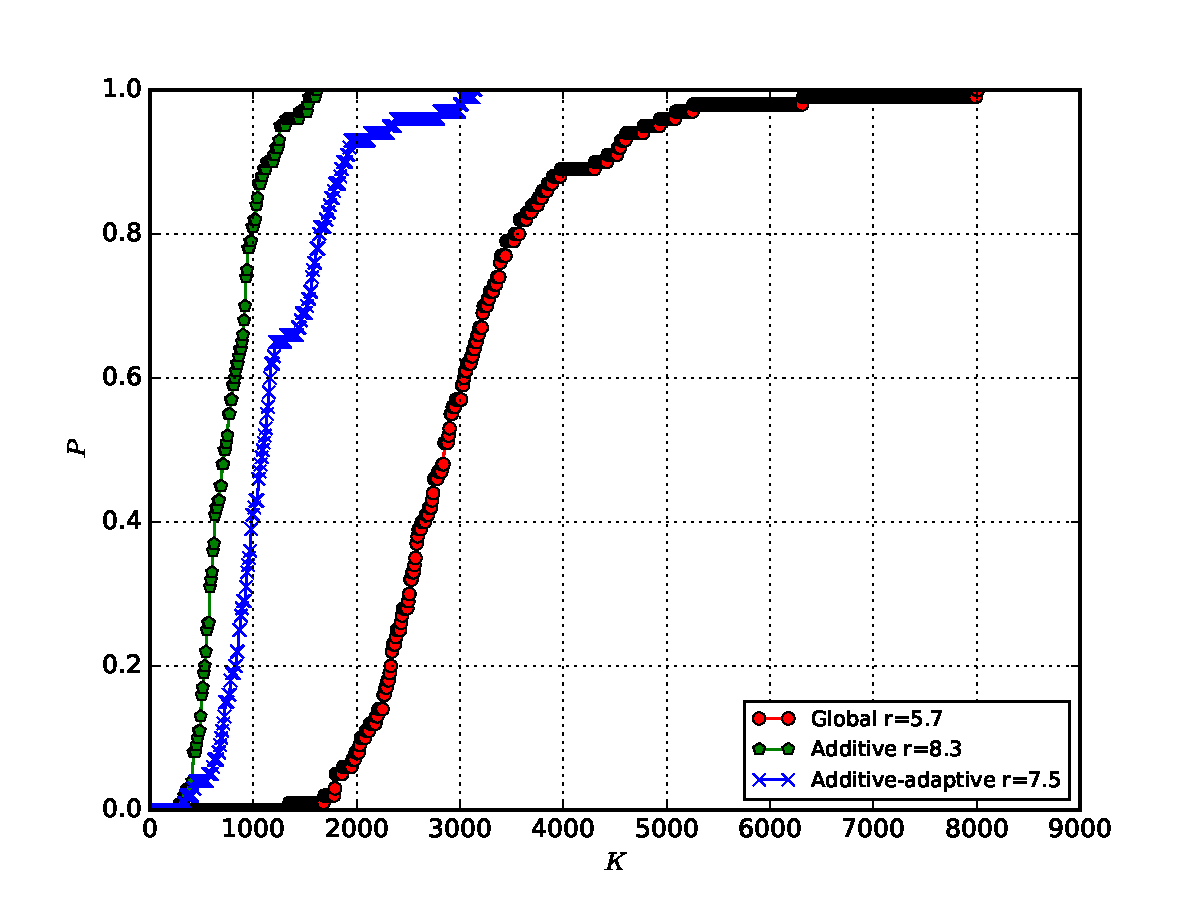
\includegraphics[width=0.75\textwidth]{images/gkls-s.pdf}
  \caption{Операционные характеристики методов на классе задач GKLS Simple 2d}
  \label{fig:gkls_op}
\end{figure}

Далее перейдём к сравнению различных вариантов метода на рассматриваемых классах задач.
В качестве оценки эффективности алгоритма будем использовать, операционную характеристику,
описанную в разделе \ref{subsec:methods_compasion}

Как видно из операционных характеристик на рис. \ref{fig:grishh_op} и \ref{fig:gkls_op},
оба метода с локально-адаптивной оценкой константы Гёльдера показали существенное преимущество, однако они требуют
задавать более высокое значение параметра \(r\). Если сравнивать между собой методы с
адаптивной и неадаптивной свёрткой (\ref{additiveConv}), (\ref{additiveAdaptiveConv}), то наглядно видно преимущество последнего,
хотя он и требует большее значение параметра надёжности \(r\) для решения задач из класса GKLS.
